\begin{frame}
  \frametitle{Hypothetical (?) scenarios}

  \begin{itemize}
  \item<1-> The computer vision subsystem of an autonomous vehicle leads the
    vehicle to take a left turn, in front of a car moving in the opposite direction\footnote{\url{https://www.theguardian.com/technology/2022/dec/22/tesla-crash-full-self-driving-mode-san-francisco}}
  \item<2-> The credit assessment system leads to the rejection of an
    application for a loan - the client suspects racial bias\footnote{\url{https://www.technologyreview.com/2021/06/17/1026519/racial-bias-noisy-data-credit-scores-mortgage-loans-fairness-machine-learning/}}
  \item<3-> A model that assesses the risk of future criminal offenses (and
    used for decisions on parole sentences) is biased against black
    prisoners\footnote{\url{https://www.propublica.org/article/machine-bias-risk-assessments-in-criminal-sentencing}}
  \end{itemize}

\end{frame}

\begin{frame}
  \frametitle{Questions}
  \begin{itemize}
  \item Why did the model make a specific decision? \textcolor{red}{local XAI}
  \item What could we change so that the model will make a different decision? \textcolor{red}{counterfactual}
  \item Can we summarize the model's behavior? \textcolor{red}{global XAI}
  \item If models are knowledge extractors, what have they learned? \textcolor{red}{global XAI}
  \end{itemize}
\end{frame}

\begin{frame}
  \frametitle{Interpretability of Machine Learning Models}
  Qualitative definitions:
  \begin{itemize}
  \item<1-> ``Interpretability is the degree to which a human can understand the
    cause of a decision'' \footnote{\href{https://arxiv.org/abs/1706.07269}{Miller (2017)}}
  \item<2-> ``Interpretability is the degree to which a human can consistently
    predict the model’s result''\footnote{\href{https://papers.nips.cc/paper/2016/hash/5680522b8e2bb01943234bce7bf84534-Abstract.html}{Kim et. al (2016)}}
  \item<3-> ``Extraction of relevant knowledge from a machine-learning model
    concerning relationships either contained in data or learned by the
    model''\footnote{\href{https://www.pnas.org/doi/10.1073/pnas.1900654116}{Murdoch et. al (2019)}}
  \end{itemize}
\end{frame}


\begin{frame}
  \frametitle{Global vs Local}
  \begin{itemize}
    \item \textcolor{red}{Global}
    \begin{itemize}
      \item Provide a general interpretation of the model's behavior
      \item Extract interpretable quantity that holds for $x \in \mathcal{X}$
      \item Example: Feature Effect $x_s \rightarrow y$
    \end{itemize}
    \item \textcolor{red}{Local}
    \begin{itemize}
      \item Interpret the model's output for a particular input
      \item Extract interpretable quantity that holds for $x$ close to $x^{(i)}$
      \item Example: Linear model that replaces $f$ around $x^{(i)}$ (LIME)
    \end{itemize}
  \end{itemize}

  \begin{figure}
    \centering
    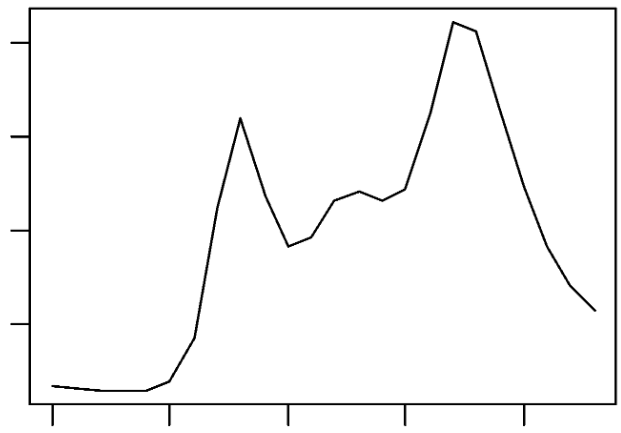
\includegraphics[width=0.37\linewidth]{ale_concept}
    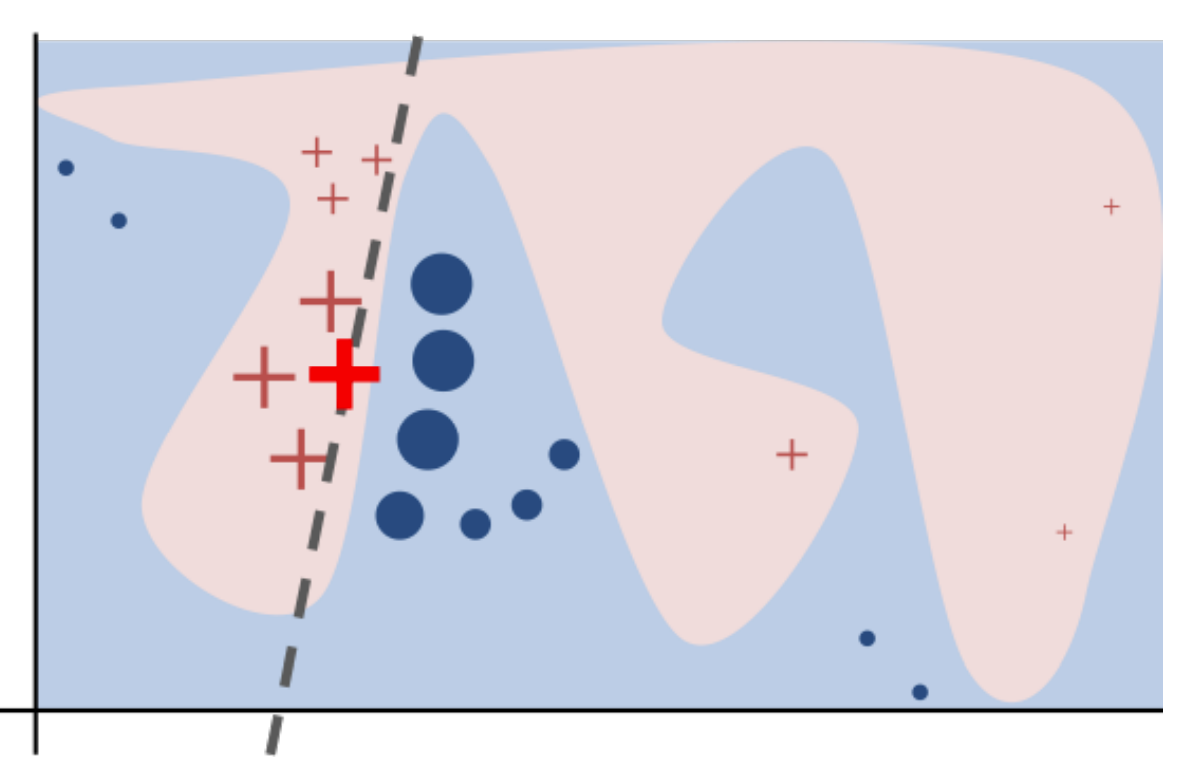
\includegraphics[width=0.4\linewidth]{lime_concept}
    \caption{(Left) Global vs (Right) Local}
    \label{fig:figure-1}
  \end{figure}
\end{frame}


\begin{frame}
  \frametitle{Advantages and challenges of global methods}

  \begin{itemize}
    \item Advantages:
    \begin{itemize}
      \item \textcolor{red}{Interpretable quantity holds for $x \in \mathcal{X}$}
      \item Global summary of the model's behavior
    \end{itemize}
    \item Challenges:
  \begin{itemize}
    \item \textcolor{red}{Interpretable quantity holds for $x \in \mathcal{X}$}
    \item Level of fidelity
    \item Level of interpretability
    \item Can we have both?
    \begin{itemize}
      \item if yes, replace the original model
      \item if no, deal with the trade-off
    \end{itemize}
  \end{itemize}
  \end{itemize}

  \noindent\makebox[\linewidth]{\rule{\paperwidth}{0.4pt}}
  if no, can uncertainty quantify the level of fidelity?
\end{frame}


\begin{frame}
  \frametitle{Methods we will discuss}

  \begin{enumerate}
  \item Feature Effect
    \begin{itemize}
      \item $1D$ plot: \(f_s(x_s): x_s \rightarrow y\)
      \item Effect (mapping) of a single feature \(x_s\) on the output \(y\)
      \item \href{https://arxiv.org/abs/1612.08468}{Apley et. al (2019)}
    \end{itemize}
  \item Feature Interaction
    \begin{itemize}
    \item Number
    \item Level of interaction between features \(x_i\) and \(x_j\)
    \item \href{https://arxiv.org/abs/1805.04755}{Greenwell et. al (2018)}
    \end{itemize}
  \item (1) + (2) $\rightarrow$ Heterogeneous Effects / Uncertainty
  \item Feature Importance
    \begin{itemize}
      \item Number
      \item To what extent the model accuracy would drop, if \(x_s\) was absent
        \item \href{https://arxiv.org/abs/1801.01489}{Fisher et. al (2018)}
    \end{itemize}

  \end{enumerate}

\end{frame}
